\vspace{-2mm}
\section{Daemon - (Broker - Server)} 

	\normalsize
	{
		The preferred name for a ``server'' in the Linux domain is ``daemon''.  The concept of a ``daemon'' is not unlike the concept of a ``server'',
		however using the term ``daemon'' negates the ambiguity associated with a ``server process'' running on a ``server computer''.  
		Throughout this section the term ``daemon'' will be used in regards to the process and the term 'server' will be used in reference to a 
		``daemon'' running on a server computer.  
		\newline
		\newline
		Furthermore the term ``broker'' creates yet more ambiguity, in that it is associated with an architectural pattern for the message validation, 
		transformation and routing.  For the sake of simplicity the term ``broker'' will be used to convey the facilitated communication 
		amongst peer processes, where a ``daemon'' in the middle between two computers facilitates this, effectively decoupling them from one another.
	}

	\vspace{3mm}
	\subsection{Requirements}
	
		\vspace{-5mm}
		\begin{multicols}{2}
		
			\begin{enumerate}[itemsep=1pt,parsep=1pt]
				\item 	Support for multiple clients			 
				\item 	Use of PERL  
				\item 	Scalable to handle 100's of clients
			\columnbreak
				\item   Master with multiple slave servers. 			
				\item   Push \& Pull technologies
			\end{enumerate}
			
		\end{multicols}
		
	\subsection{Technologies}
	
		\vspace{-5mm}
		\begin{multicols}{2}
		
			\begin{itemize}
			
				\item \textbf{PERL threads}	
					\newline								
					PERL threads were used extensively in the application for the client server model to gain maximum performance.  
				
				\item \textbf{PERL threads::shared}	
					\newline								
					To shared variables amongst threads.
										
				\item \textbf{PERL Thread::queue}	
					\newline								
					Queues were used extensively in both the client and the server.  The server has an incoming queue,
					processing queue and an outgoing queue.  The queues are thread safe and are first come first served basis
					ensuring ordered processing.
							
				\item \textbf{PERL Thread::Semaphore}	
					\newline								
					Certain critical sections in the client and server where identified and errors avoided by using semaphores.
					
		\columnbreak			
					
				\item \textbf{PERL IO::Socket}	
					\newline								
					A low level socket implementation was preferred for maximum performance.				
					
				\item \textbf{PERL POSIX}	
					\newline								
					Portable Operating System Interface (POSIX) was used in the application for the signalling of 
					threads and user interrupts which is a small subset of the POSIX API.  
					
				\item \textbf{PERL JSON}	
					\newline								
					For message passing in the implementation between the nodes this was the preferably choice for message passing.
						
				\item \textbf{PERL Sys::Syslog}		
					\newline							
					Syslog the de-facto means of logging in Linux and as such the choice to use Sys::Syslog 
					to log client - server interactions was required.
					
				\item \textbf{PERL DBI}			
					\newline						
					This database abstraction layer decouples the programmer from specific database API.   As it is a wrapper
					a common database connection string is used to specify the database type and the abstraction layer takes care of the specific
					API calls.  As such this allows for the use of most common database technologies, such as hierarchical, relation and object 
					oriented databases.
					
			\end{itemize}	
			
		\end{multicols}
	
	\subsection{Design}
			
		\normalsize
		{
			Although not subscribing to any particular design when designing the client server architecture,
			there were multiple influencing sources that lead to the architecture shown in Fig. \ref{fig:ServerQueues}.
			The book \textit{Pattern Oriented Software Architecture - Patterns for concurrent and networking objects} was a key 				
			influence on this simplified design, specifically with reference to the key aspects of the ``interceptor'' and ``leader / followers''
			design patterns.
			
			\noindent\begin{minipage}{\textwidth}
			
				\begin{figurehere}
					\centering
					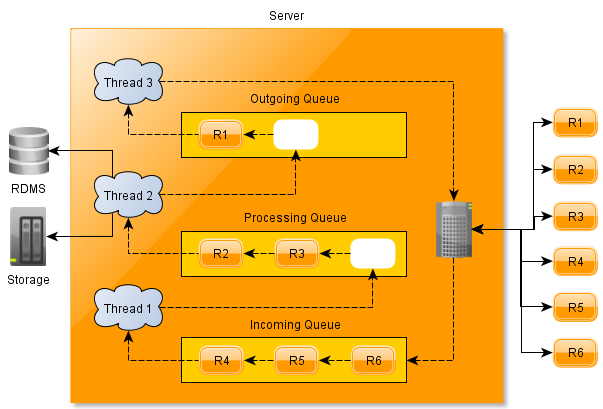
\includegraphics[scale=0.7]{pages/chapter3/figures/server-marchitecture.png}
					\caption{Server Queues}
					\label{fig:ServerQueues}
				\end{figurehere}	
			
			\end{minipage}
			
			\vspace{5mm}
			The architecture presented shows (R)equests moving through the internal data lanes of the implementation.
			Three queues are the main transition points within the architecture, namely the incoming, processing and 
			outgoing queues and the associated threads 1, 2 \& 3.  
			These requests internal messages can be divided into two major categories, Administrator and Client requests.
						
			\vspace{-3mm}
			\begin{multicols}{2}	
			
				\begin{itemize}[itemsep=1pt,parsep=1pt]
					\item \textbf{Administrator Requests}
						\begin{itemize}
							\item Module List
							\item Save / Update Module
							\item Synchronise Policies
							\item Push Policies to clients 
							\item Push Modules to clients
						\end{itemize}
				
				\columnbreak
						
					\item \textbf{Client Requests}
						\begin{itemize}
							\item Module Update
							\item Policy Update
						\end{itemize}					
				\end{itemize}	
				
			\end{multicols}	
			
			Although not immediately indicated the requests are asynchronous, meaning that the connection to the client
			is dropped as soon as the request is accepted.  By analysing the diagram we can also see that the queues enforce 
			the ordering of the events and subsequent resource interaction, such as database access or disk access.
			\newline
			\newline				
			The incoming queue is important as requests must be handled as fast as possible when implementing a server.
			If too many connections to a socket are open (IP address bound to a port eg. 127.0.0.1:80) there is the
			possibility of the server reaching the maximum allowed by the operating system.  This in turn this would give a busy
			signal to the subsequent clients trying to connect.  Connections that are accepted are immediately inspected
			for its request and this request is put into the incoming queue.  Finally thread 1 is responsible for determining
			whether the messages is well formed before being placed into the processing queue.				
			\newline
			\newline
			The processing queue is the next main transition for a request. In the processing queue the requests internal 
			message is analysed by thread 2 and subsequent processing is done depending on the request.  
			Once the processing is complete the request is put into the out going queue.	
			\newline					
			\newline
			Finally Thread 3 and the associated outgoing queue is responsible for sending a response back to the client/administrator 
			where applicable.  It is worth point out at this stage that the envelope in which the request is encapsulated, 
			holds information such as the peer IP address, peer port, peer request etc.
			\newline
			\newline
			With this information and the daemon response inserted into the request envelope by thread 2, 
			the outgoing queue is then processed by thread 3.  Thread 3 opens a connection to the destination and sends the response
			to the requester.					
		}				

	\vspace{4mm}
	\subsection{Architecture}
		\label{sec:serverarch}
		
		\normalsize
		{
			An introduction to software architecture by \citet{introsoftwarearchitecture} makes reference to state transitions 
			as an important aspect of the architectural design.  Fig. \ref{fig:ServerQueues} on the previous page
			offers three primary state transitions.  
			
			\vspace{-5mm}
			\begin{multicols}{3}
			
				\begin{itemize}[itemsep=1pt,parsep=1pt]
					\item \textbf{Incoming}				
					\item \textbf{Processing}		
					\item \textbf{Outgoing}	
				\end{itemize}	

			\end{multicols}		

			As a request passes through these data lanes or queues, the action of moving from one state to another
			offers pre marshalling and post marshalling capabilities.  We can extend the transitions as follows :
			
			\vspace{-2mm}
			\begin{multicols}{3}
			
				\begin{itemize}[itemsep=1pt,parsep=1pt]
				
					\item Incoming	
						\begin{itemize}
							\item \textbf{Pre incoming}				
							\item \textbf{Post incoming}	
						\end{itemize}
						
						
					\item Processing	
						\begin{itemize}
							\item \textbf{Pre processing}				
							\item \textbf{Post processing}	
						\end{itemize}
						
					\item Outgoing	
						\begin{itemize}
							\item \textbf{Pre outgoing}				
							\item \textbf{Post outgoing}	
						\end{itemize}
						
				\end{itemize}
				
			\end{multicols}				
		
			Each of these states offers transition points and the ability to include extensions to the framework
			to target specific requirements.  As an example of this, the implementation of the architecture allows for the addition
			of different security extensions for the both the pre incoming and pre outgoing transitions.
			In an example scenario an encrypted request that has been accepted into the incoming queue must first be decrypted
			before processing of the encrypted data can be accomplished.  Similarly the encryption of the outgoing response
			can be handled at the pre outgoing transition.  The following eight steps presented can be are identified in Fig. \ref{fig:Transitionstatesmarshalling}.
			\newline
			
			\begin{enumerate}[itemsep=1pt,parsep=1pt]
				
				\item Encrypted peer request is received			
				\item Request is added to the incoming queue	
				\item Thread 1 processes next request on the incoming queue
				\item Encryption extension decrypts message \textbf{(pre marshalling)}
				\item Thread 1 places decrypted request into processing queue \textbf{(post marshalling)}
				\item Thread 3 processes next item on out going queue
				\item Encryption takes place on the out going message \textbf{(pre marshalling)}
				\item Thread 3 sends the message to the peer \textbf{(post marshalling)}
				
			\end{enumerate}
					
			\vspace{4mm}
			This concept of pre and post marshalling effectively allows for the integration of different extensions to cover a multitude of
			future requirements and upgrades. These extensions could provide concepts such as load balancing, priority queues,
			multi-threaded queues and integration with other directory service systems.  
			\newline
			\newline
			Due to the time constraints of the project the decision to implement the daemon in this fashion provides the ability
			to satisfy the requirement of a master slave paradigm.  In an example scenario, the master server could provide load balancing
			by re routing incoming requests to slave daemons running on other servers. The potential resource heavy and time sensitive processing operation
			is then passed and balanced among these slave servers.  
			\newline
			
			\vspace{-3mm}
			\noindent\begin{minipage}{\textwidth}
				
				\begin{figurehere}
					\centering
					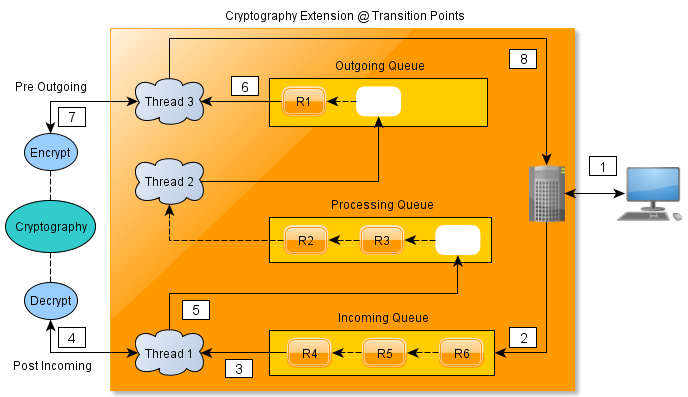
\includegraphics[scale=0.65]{pages/chapter3/figures/servertranitionstates.png}
					\caption{Transition states marshalling}
					\label{fig:Transitionstatesmarshalling}
				\end{figurehere}	
			
			\end{minipage}
		}
		

\newpage
		
	\subsection{Coding} 		
	
		\normalsize
		{
			The discussion of the design and architecture covers the following five technologies. These cover the basic concepts of threading and critical sections, first in first out (FIFO) queueing data structures
			and key concepts of socket programming. 
		}			
		
		\begin{itemize}[itemsep=1pt,parsep=1pt]
			\item \textbf{PERL threads}					
			\item \textbf{PERL threads::shared}				
			\item \textbf{PERL Thread::queue}	
			\item \textbf{PERL Thread::Semaphore}				
			\item \textbf{PERL IO::Socket}			
		\end{itemize}
			
					
		\normalsize
		{
			All of these topics are huge topics in themselves and are well understood fundamentals in computer science.  
			Therefore in this section I'm going to cover the more opaque technologies and provide coding snippets
			to support the reasoning for the choice of these technologies.
			\newline
		} 
		
			\begin{itemize}[itemsep=1pt,parsep=1pt]
				\item \textbf{PERL POSIX}						
				\item \textbf{PERL JSON}	
				\item \textbf{PERL Sys::Syslog}							
				\item \textbf{PERL DBI}							
			\end{itemize}
			
		\vspace{3mm}
		\large{\bfseries{POSIX}}
		
		\normalsize
		{
			The Portable Operating System Interface (POSIX) is an application programmers interface for maintainability compatibility between operating systems.  
			The use of POSIX in the implementation was primarily used for thread signalling and ensuring the clean shut down of the daemon.  
			\newline
			\newline
			In order to communicate with the daemon from an administration point of view
			where an administrator is logged onto the server some sort of inter-process communication is required.  For example, 
			rather than abruptly killing the server daemon with a ``kill -9 daemon'' command, named pipes were
			used to send this messages to the daemon.
			\newline
			\newline
			Named pipes are a basic form of inter process communication in Unix, Linux, Windows and Mac operating systems, however the semantics and resulting implementations differ.
			In Unix the implementation of this concept is achieved via use of the file system.  
			\newline
			\newline
			The mkfifo command on Unix and derivative platforms, makes use of the POSIX API to signal the kernel to
			prepare a file on the file system that acts as a first in first out queue, for inter process communication.  Piping information into this file is placed in shared memory. 
			The receiving process can then read this file (effectively the memory) achieving inter process communication.
			An example of this is given in Fig \ref{fig:perlreatepipe}.
		}
		
\newpage
						
		\begin{figurehere}
			\inputminted[linenos=true,fontsize=\footnotesize,tabsize=2]{perl}{pages/chapter3/smippets/perlfifo.pl}
			\vspace{-2mm}
			\caption{Creating and reading a named pipe}
			\label{fig:perlreatepipe}
		\end{figurehere}
		
		\vspace{5mm}
		\normalsize
		{
			In this example a named pipe is created and then opened for reading and writing.  As soon as data is piped into the file, this line is read using the chomp Perl function.
			The line is inspected for keywords, in this case ``stop'' and the internal variable ``continue'' is set to minus one.  All other threads within the application
			implement looping constructs based upon this ``continue'' variable.  When ``continue'' it is set to minus one,  this loop constructs discontinue, illustrated by the coding snippet in Fig. \ref{fig:perlqueues}.
		} 
				
		\begin{figurehere}
			\inputminted[linenos=true,fontsize=\footnotesize,tabsize=2]{perl}{pages/chapter3/smippets/threadscont.pl}
			\vspace{-2mm}
			\caption{Threads discontinue processing}
			\label{fig:perlqueues}
		\end{figurehere}
		
		\vspace{4mm}
		\normalsize
		{
			The second use of signalling is for the scenario where interrupts such as a kill signal is sent to the daemon process.
			As an example I will provide a simple scenario of running the daemon in the shell console context. Typically when a daemon is launched from within
			the context of a shell it detaches itself from the console.  However if it does not do this, when the shell is finished or is closed 
			it kills any processes which it has launched.  This concept is familiar to programmers
			who write managed code where the garbage collector removes unused or unreferenced artefacts in memory.
			\newline
			\newline
			Running a daemon in the shell context present a problem.  Cleanly shutting down the process is important when the cancel or kill signal is fired.
			This is typically done on systems using ``CTRL \textasciicircum  C''.  To ensure clean shut down and the termination of threads, this signal must be ``caught''.
			Threads must be told to shut down and finally terminate the program.
			\newline
			\newline
			This is accomplished via POSIX,  terminals typically implement POSIX and encompassing signalling.  So when ``CTRL \textasciicircum  C'' is 
			pressed the terminal catches the signal and terminates the application.  Therefore we must intercept this signal and handle this terminal event.  
			PERL provides POSIX support and with this we can intercept the kill signal;  Fig. \ref{fig:perlsignals} presents this.
			\newline
		} 
		
		\begin{figurehere}
			\inputminted[linenos=true,fontsize=\footnotesize,tabsize=2]{perl}{pages/chapter3/smippets/signals.pl}
			\vspace{-5mm}
			\caption{PERL Signals}
			\label{fig:perlsignals}
		\end{figurehere}
		
		\vspace{3mm}		
		\normalsize
		{
			In this example ``SIG'' which is a global variable provided by the POSIX module in PERL provides a means to map a signal to a closure
			or method stub.  When the ``INT'' signal is received the ``signal\_interrupt'' is called which tells the server to shut down.  
			In order to override repeated ``CTRL \textasciicircum  C'' events we re-map the INT signal once again to the ``signal\_interrupt'' closure.
			Finally the client sleeps for 1 second, this typically will allow threads to shut down before the application terminates.
			\newline
			\newline
			Context switches in the kernel are guaranteed to be no more than 500ms. This duration allows all attached threads
			to shut down or terminate before the application exits.  Typically in a modern processor, context switches can occur up
			20,000 times per second. This means that this amount of threads could be terminated in this time allotment. In the implementation
			the stop method in the daemon class has more than enough time to achieve this goal.  An excerpt of this stop method is provided in Fig. \ref{fig:StopServerThreads}.
		} 
		
		\vspace{2mm}
		\begin{figurehere}
			\inputminted[linenos=true,fontsize=\footnotesize,tabsize=2]{perl}{pages/chapter3/smippets/serverstop.pl}
			\vspace{-4mm}
			\caption{Stop Server Threads}
			\label{fig:StopServerThreads}
		\end{figurehere}
		
\newpage

		\large{\bfseries{JSON}}	
		
		\normalsize
		{		
			Javascript Object Notation (JSON) is a lightweight data-interchange format for the transfer of platform independent communication.  
			The name may suggest that it is for Javascript only, however most of the 3rd and 4th generation programming languages implement JSON parsers.  
			The choice of JSON over the typically used Extensible Markup Language(XML) was the syntactic verbosity factor.  There are examples on json.org that indicate
			XML can be 300\% more verbose than JSON.  In a system that is dependent on speed and efficiency, the smaller and hastily parsing of messages is important.
			Therefore JSON was a good candidate for encapsulation of messages due to its' lightweight envelope.  Initially I had devised my own short form syntax for messages
			however as the implementation grew and the message became more complex, the need for a better envelope and formatting of messages was required.
		}
		
		\vspace{2mm}
		\begin{figurehere}
			\inputminted[linenos=true,fontsize=\footnotesize,tabsize=2]{perl}{pages/chapter3/smippets/jsonmessage.pl}
			\vspace{-2mm}
			\caption{JSON Client Request}
			\label{fig:ClientJsonRequest}
		\end{figurehere}
				
		\normalsize
		{	
			In section \ref{sec:serverarch} identified the messages that the server dealt with, one of them being a client update.  
			As an example Fig \ref{fig:ClientJsonRequest} presents a request from a client for a policy update.  The key ``request'' holds the value
			or the intended request to be sent to the server.
			\newline
		}
		
		\large{\bfseries{Syslog}}	
		
		\normalsize
		{		
			Syslog is a data logging standard used by Unix and derivatives as a means to decouple processes from operating system logging mechanism.
			These logs can then be checked by administrators of the environment and reports made from them.  In order to debug daemons where the standard output is not visible
			as the daemon is not attached to a console, a means of logging messages is required.  The integration with the system implementation logging features
			is expected and as such the choice for Syslog was mandatory.
			\newline
			\newline
			An entry is made into the Syslog configuration.  The entry is then used to create a pipe by Syslog to which process can redirect messages to; 
			 resulting in the corresponding file.
			\newline
			\begin{center}
			local6.*						/var/log/lgp
			\end{center}
			\vspace{5mm}
			The following PERL excerpt in Fig. \ref{fig:PerlSyslog} shows the use of this logging mechanism and the corresponding log file excerpt below it.
		}
				
		\begin{figurehere}
			\inputminted[linenos=true,fontsize=\footnotesize,tabsize=2]{perl}{pages/chapter3/smippets/syslog.pl}
			\vspace{-2mm}
			\caption{PERL Syslog}
			\label{fig:PerlSyslog}
		\end{figurehere}
		
		\vspace{5mm}
		\normalsize
		{
			Mar 29 17:16:25 testmachine2 cmain.pl[3657]: Client created tcp connection on 192.168.1.10:50000
			\newline
		}
						
		\large{\bfseries{DBI}}	
		
		\normalsize
		{					
			As the back end of the architecture depends on database for storage, a major concern is the subscription to a vendor specific database.
			This vendor database may in the future be deprecated and the need to migrate to a new database vendor may occur.
			The PERL DBI (PERL Database Interface) offers an abstraction for programmers using the PERL programming language from vendor specific
			database implement ion application programmer interfaces.  Programmers who are familiar with connection strings such as that used in .NET of ODBC will be 
			familiar with this concept.  Other languages such as PHP provide the PHP Data Objects (PDO) as a comparable abstraction.  
			This abstraction layer allows for the choice of database based upon a connection string.
			In Fig. \ref{fig:Perldbi} the connect stub of the database PERL module in the implementation provides the ability to change the database type
			at rune time.
		}
		
		\vspace{2mm}
		\begin{figurehere}
			\inputminted[linenos=true,fontsize=\footnotesize,tabsize=2]{perl}{pages/chapter3/smippets/dbi.pl}
			\vspace{-2mm}
			\caption{PERL DBI}
			\label{fig:Perldbi}
		\end{figurehere}	 
		
\newpage
	
	\subsection{Analysis}
	
		\normalsize
		{					
			Many concerns arise when attempting to do an analysis of the daemon; namely speed, scalability, extensibility, maintainability, 
			portability and security.  There are many topics.  In this analysis I'm going to tackle the speed concerns, and the resulting scalability. 
			\newline
			\newline
			Stress testing was done on the implementation as a means to elicit empirical evidence to validate the requirements, namely
			``Scalable to handle 100's of clients''.  A stress test harness was setup to address this concern.  The stress test consisted of six virtual machines, 
			one server and five clients running on a single computer.	Table \ref{tab:TestMachine} presents the test machine characteristics.
			\newline
		}
		
		
		\begin{tablehere}	
		
			\begin{tabular}{rrrr}

				{\bf Test Machine} 						& {\bf Cores} 	& {\bf Threads} 		&            		\\ \hline
				{\bf Intel Core I7 965 @ 3.2 GHZ} 		&          4 	&          8 			&            		\\
														&            	&            			&            		\\
														&  {\bf Ram} 	&            			&            		\\ \hline
				{\bf DDR3 PC3-10666 Triple Channel } 	& 16 Gigabytes 	&            			&            		\\
														&            	&            			&            		\\
														& {\bf IOPS} 	& {\bf Form Factor} 	&  {\bf RPM} 		\\ \hline													
				{\bf OCZ RevoDrive } 					&      70000 	& PCI-Express RamDrive 	&        N/A 		\\
														&            	&            			&            		\\
				{\bf Vmware Virtual Machines} 			&  {\bf Ram} 	& {\bf Threads} 		& {\bf Function} 	\\ \hline
				{\bf Redhat 32} 						& 2 Gigabytes 	&          2 			&     Daemon 		\\
				{\bf Fedora 32} 						& 2 Gigabytes 	&          2 			&     Client 		\\
				{\bf Fedora 64} 						& 2 Gigabytes 	&          2 			&     Client		\\
				{\bf Gentoo} 							& 2 Gigabytes 	&          2 			&     Client 		\\
				{\bf Ubuntu} 							& 2 Gigabytes 	&          2 			&     Client 		\\
				{\bf Open Suse} 						& 2 Gigabytes 	&          2 			&     Client 		\\

			\end{tabular}  
			
			\caption{Test Machine}
			\label{tab:TestMachine}
			
		\end{tablehere}	
		
		\vspace{5mm}
		\normalsize
		{					
			It was important to negate all possible bottle necks in the test equipment.  To achieve characteristics of 
			enterprise level server performance. I negated the hard drive bottle neck that would be associated with personal computers.
			As in an enterprise environment, ``filers'' would be used as a data centres backbone for storage; due to their high performance.
			\newline
			\newline
			Making the comparison between OCZ RevoDrive in table \ref{tab:TestMachine} and that of consumer grade hard drive is presented
			in table \ref{tab:HardDrivesComparison}.  The form factor presented indicates approximately 14 times faster hard drive access speed.
			\newline
		}
		
		
		\begin{tablehere}	
		
			\begin{tabular}{rrrr}

				{\bf Comparison} 						& {\bf IOPS} 	& {\bf Form Factor} 	&  {\bf RPM} 		\\ \hline
				Sata 3 Hard Drive  						&        150 	& Sata 3 HDD 			&       7200 		\\
				Sata 3 Solid State Drive 				&       5000 	& Sata 3 SSD 			&        N/A 		\\

			\end{tabular}  
			
			\caption{Hard Drives Comparison}
			\label{tab:HardDrivesComparison}
			
		\end{tablehere}	
		
\newpage		
		
		\normalsize
		{					
			The test composed of 500 requests to the daemon to push out updates to the clients, each with a delay of 30ms between each request. 
			In effect this meant that there were 500 + (5 * 500) equalling 3000 asynchronous requests.
			\newline
			\newline
			A sampling interval of 1 second was used to capture information, such as processor, queueing and network loads.
			The resulting data is shown in Fig. \ref{fig:ServerCpuUsage}, \ref{fig:ServerQueueUsage} and \ref{fig:ServerNetworkUsage} respectively.
			\newline
		}		
		
		\noindent\begin{minipage}{\textwidth}
			
			\begin{figurehere}
				\centering
				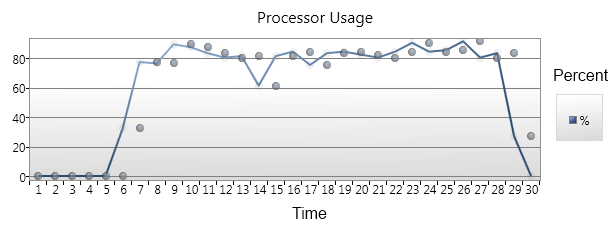
\includegraphics[scale=0.9]{pages/chapter3/figures/server-cpu.png}
				\vspace{-2mm}
				\caption{Server CPU Usage}
				\label{fig:ServerCpuUsage}
			\end{figurehere}	
		
		\end{minipage}
		
		\vspace{6mm}
		\noindent\begin{minipage}{\textwidth}
			
			\begin{figurehere}
				\centering
				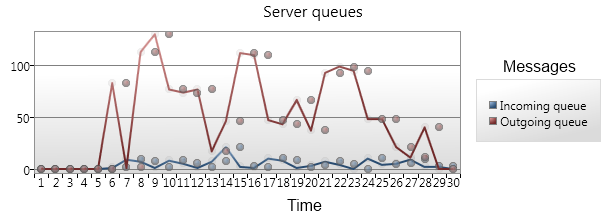
\includegraphics[scale=0.9]{pages/chapter3/figures/server-queues.png}
				\vspace{-2mm}
				\caption{Server Queues Usage}
				\label{fig:ServerQueueUsage}
			\end{figurehere}	
		
		\end{minipage}
		
		\vspace{6mm}
		\noindent\begin{minipage}{\textwidth}
			
			\begin{figurehere}
				\centering
				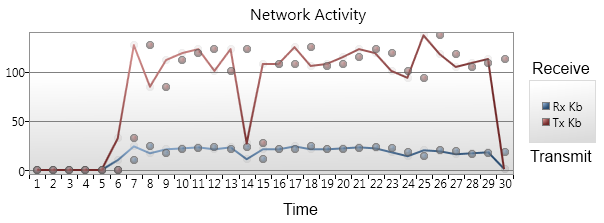
\includegraphics[scale=0.9]{pages/chapter3/figures/server-network.png}
				\vspace{-2mm}
				\caption{Server Network Usage}
				\label{fig:ServerNetworkUsage}
			\end{figurehere}	
		
		\end{minipage}
			
		\vspace{5mm}
		\normalsize
		{					
			The test took approximately twenty five seconds, equaling one hundred client updates per second.  In the implementation however,
			the client checks for updates every twenty minutes.  As there is 1200 seconds in this time, potentially under 
			optimal conditions the server could handle 120,000 clients.  This hypothetical scenario is based upon a policy
			that equates to approximately one kilobyte and optimal testing conditions.  
			Under real conditions this scenario may not be feasible, due to larger policies and possible network degradation. 
			The achievement of 5\% of this performance this still equates to approximately six thousand client updates, in this twenty minute interval.		
			\newline
		}	
			
	
	\subsection{Improvements}

		\normalsize
		{					
			In \textit{Patterns of Enterprise Application Architecture} by Martin Fowler, he makes numerous references to case studies were 
			performance testing presented bottle necks in string processing.  The resulting degraded application performance was in some cases
			diabolical and light weight changes resulted in 100\% increased efficiency.  
			In the server architecture the daemon makes use of numerous text conditionals and JSON.  Ultimately these text conditionals need to be
			lexicographically parsed, resulting in high processor usage as indicated by figure \ref{fig:ServerCpuUsage}.
			\newline			
			\newline
			To begin to target this contention in future improvements, the use of JSON as an envelope for message passing might be dropped.
			Initially during development I did not use JSON, however as the complexity grew a need for a structured message was required, as sequenced
			events became difficult to maintain.
			\newline
			\newline
			Furthermore as the client sends requests as text, these text conditionals need to be lexicographically inspected and compared
			by the daemon to create the correct response.  These text conditionals could be replaced by integer values
			that require very little computation in terms of comparison by a processors arithmetic logic unit (ALU).  
			\newline
		}	

	
	
	
	
	
	
	
	
	
	
	
	
	
	
	


\section{Client} 

	\normalsize
	{
		In this section the discussion of the client; it's operations and supporting technologies will be consummated.
		along with a brief introduction to the transliteration of the domain specific language.
		\newline
		\newline
		The client implementation is responsible for downloading a policy from the daemon and executing it.
		The execution of the policy, a domain specific language (DSL) is the application of the rules defined by the administrator.
		The client determines the operating system distribution it is executing on and through the use of an interpreter, it applies the policy  
		via distribution specific commands.  
	}

	\vspace{3mm}

	\subsection{Requirements}
	
		\begin{enumerate}[itemsep=1pt,parsep=1pt]
		
			\item 	Support for multiple distributions
			\item 	Client must be extensible
			\item 	Use of PERL 
			\item 	Updates to varying architectures
			\item   Push \& Pull technologies
			
		\end{enumerate}
		
	\subsection{Technologies}
	
		\vspace{-5mm}
		\begin{multicols}{2}
			
			\begin{itemize}
			
				\item \textbf{PERL threads}	
					\newline								
					PERL threads were used extensively in the application for the client server model to gain maximum performance.  
				
				\item \textbf{PERL threads::shared}	
					\newline								
					To shared variables amongst threads.
					
				\item \textbf{PERL Thread::queue}	
					\newline								
					Queues were used extensively in both the client and the server.  The server has an incoming queue,
					processing queue and an outgoing queue.  The queues are thread safe and are first come first served basis
					ensuring ordered processing.
					
				\item \textbf{PERL Thread::Semaphore}	
					\newline								
					Certain critical sections in the client and server were identified and errors avoided by using semaphores.
					
				\item \textbf{PERL IO::Socket}	
					\newline								
					A low level socket implementation was preferred for maximum performance.				
					
				\item \textbf{PERL POSIX}	
					\newline								
					Portable Operating System Interface (POSIX) was used in the application for the signalling of 
					threads and user interrupts which is a small subset of the POSIX API.  
							
				\item \textbf{PERL JSON}	
					\newline								
					For message passing in the implementation between the nodes this was the preferably choice for message passing.
				
				\item \textbf{PERL Sys::Syslog}		
					\newline							
					Syslog the de facto means of logging in Linux is assumed by all major daemon installations
					and as such the choice to use Sys::Syslog to log client server interactions was required.
					
				\item \textbf{PERL Filter::Simple}	
					\newline								
					Source filtering or pre processing is an immensely powerful feature of PERL. 
					Effectively, it allows or provides the ability to create micro languages such as a DSL by
					preprocessing the input script translating it as necessary.
					
			\end{itemize}	
		
		\end{multicols}	
	
	\subsection{Design \& Architecture}
							
		\normalsize
		{
			The client operates in the same way as the server architecture shown in Fig. \ref{fig:ServerQueues} with the minor exceptions.
			The two main differences of the client are the messages and the operations done within the in the processing queue.
			The design analysis in this section will be therefore focused upon these operations and the encompassing interpreter.  
			As the interpreter facilitates the parsing of the domain specific language (DSL) resulting in distribution specific commands, 
			the resulting architectural design evolved to support the extensibility of this framework and the interpreter.
			Fig. \ref{fig:ClientInterpretor} presents a high level design overview. 
			\newline

			\noindent\begin{minipage}{\textwidth}

				\begin{figurehere}
				\centering
				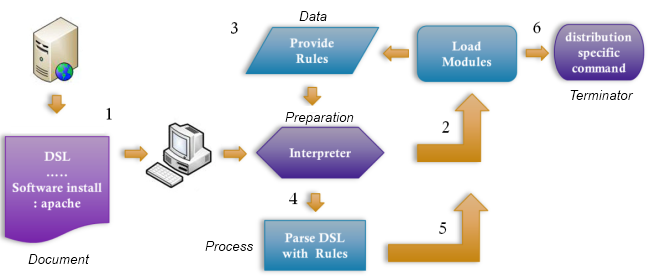
\includegraphics[scale=0.9]{pages/chapter3/figures/cleintmarchitecture.png}
				\caption{Client Interpreter}
				\label{fig:ClientInterpretor}
				\end{figurehere}	

			\end{minipage}
			
			\vspace{5mm}
			The marchitecture or control flow diagram (simplified) here presents the major sequences of events
			leading to a policy (set of rules) application.  A Unified Modelling Language (UML) Diagram is presented in 
			\ref{fig:InterpretorFramework} in Appendix 3.  
			
			\vspace{-3mm}
			\begin{multicols}{2}
			
				\begin{enumerate}
			
					\item \textbf{Receive policy update}	
						\newline								
						Server sends a policy update in the form of a domain specific language 
					
					\item \textbf{Interpreter initialises}	
						\newline								
						The interpreter is executed and loads the interpreter extensions (PERL modules)
						
					\item \textbf{Modules provide parsing rules}	
						\newline								
						The module(s) provide lexicographical parsing rules for the interpreter
						
					\item \textbf{Policy is parsed}	
						\newline								
						The interpreter parses the domain specific language (policy) using the parsing rules
						
				\columnbreak
						
					\item \textbf{lexicographically accepted lines are sent back to the modules}	
						\newline								
						For each successful line parsed, this line is sent back to the PERL module that provided the rule			
						
					\item \textbf{Module performs distribution specific command}	
						\newline								
						Further inspection is done on the line, eventually resulting in a distribution specific command				

				\end{enumerate}	
				
			\end{multicols}
		}		

		\normalsize
		{
			Unlike the server architecture, the messages can only come from the server to which the client is bound.
			There is no direct communication between the administrator interface and the clients, hence the concept of the broker.
			As an example, if the administrator sends  \textit{Push Policies} to the server, then the server iterates the known or 
			bound clients and pushes out the policy in the form of the DSL to the clients.
			\newline
			\newline				
			The client messages are as follows :
			
			\vspace{-3mm}
			\begin{multicols}{2}
			
				\begin{enumerate}[itemsep=1pt,parsep=1pt]
					\item \textbf{Request Policy Update}
					\item \textbf{Receive Policy Update}
					\item \textbf{Request Modules Update}
					\item \textbf{Receive Modules Update} 
				\end{enumerate}	
				
			\end{multicols}

			These messages provide a second point of interest from an administrator perspective.
			How does an administrator easily update the client and the interpreter modules?
			In a large enterprise environment updating the client with new modules via typical software installation
			means, ie. sitting at the computer and updating it, which is not feasible.  Any software extensibility provided by the client
			would be potentially negated by this time consuming operation.   Therefore the design to support extensibility
			has been bolstered by the ability to push out new client modules and updates. 
			\newline			
			\newline
			These modules are kept on the same server as the daemon.  The clients check for modules updates at set intervals.
			To reduce network traffic a checksum of each module is sent to the client. The client compares this checksum against it's local copy.
			If there is a difference, an update has occurred and this modified or new module is requested by the client from the daemon.
			\newline
			\newline
			This allows the administrators to create and modify modules on a continual basis, thereby meeting the enterprise specific 
			regulations and requirements, that can subject to change on a continual basis.
			\newline
		}		
	
	\subsection{Patterns}
	
		\normalsize
		{
			As previously discussed the modules have two primary functions :  
			
			\begin{itemize}[itemsep=1pt,parsep=1pt]
				\item \textbf{To extend the interpreter and the language that it understands }
				\item \textbf{The Interpretation of rules, resulting in distribution specific commands}
			\end{itemize}				
		}
			
			\vspace{-3mm}
			\begin{multicols}{2}
			
				Administrators who intend to implement new modules are implementing observers as seen in the Observer Design Pattern, Fig. \ref{fig:ObserverDesignPattern}.
				\newline
				\newline
				These observers provide new grammar to the interpreter, which in turn sends updates, using the Observer Design Pattern update mechanism. 
				Each individual rule(line) that is accepted by the interpreter using the provided grammar rules, is sent to all modules.	
				Each module knows if this update is detonated for it, as it has provided the rule to the interpreter.
			
				\columnbreak
				
				\begin{figurehere}
					\centering
					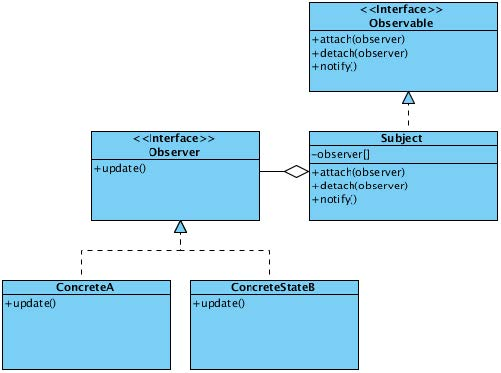
\includegraphics[scale=0.55]{pages/chapter3/figures/observer.jpg}
					\caption{Observer Design Pattern}
					\label{fig:ObserverDesignPattern}
				\end{figurehere}
			
			\end{multicols}
			
		\normalsize
		{			
			This offers the ability to provide modules outside of this preordained behaviour.  Modules could be designed to
			monitor, log or validate these messages and their outcomes.  This one to many relationship (policy line to modules) does create a 
			little extra processing, however, it provides more flexibility for administrators creating modules.  A module that has too many responsibilities
			may become difficult to maintain, therefore the separation of logging, monitoring \& validating into different modules are handled
			by this design decision.
			\newline
		}	
		
\newpage
	
	\subsection{Coding} 
	
		Dissecting the domain specific language (DSL) in Fig. \ref{fig:DSL},  we can see at the beginning the interpreter is included.  
		The interpreter which will eventually go on to read the DSL, firstly constructs the framework which in turns loads the modules.
		
		\vspace{4mm}
		\begin{figurehere}
			\inputminted[linenos=true,fontsize=\footnotesize,tabsize=2]{perl}{pages/chapter3/smippets/dsl}
			\vspace{-5mm}
			\caption{DSL}
			\label{fig:DSL}
		\end{figurehere}	
			
		\vspace{4mm}
		During the loading of the modules, the ``registerGrammer'' method is called on each module (Fig. \ref{fig:Loadmodules}).  
		There is pure assumption from module loader that module being loaded provides a new method and a ``registerGrammer'' method.
		This reflects the concept of late binding,  unlike the early binding method of using reflection to firstly inspect an object for a method
		and binding appropriately.
		
		\vspace{4mm}
		\begin{figurehere}
			\inputminted[linenos=true,fontsize=\footnotesize,tabsize=2]{perl}{pages/chapter3/smippets/loadmodules}
			\vspace{-5mm}
			\caption{Load modules - Simplified}
			\label{fig:Loadmodules}
		\end{figurehere}	
		
		\vspace{4mm}
		There are of course positive and negative effects of this.  As PERL has run time flexibility as seen in most interpreted languages.  
		Up front validation of the module implementation is difficult requiring a try and test approach of module development.  
		This would not be advisable in a live environment and should be done in a test harness,  a group of machines separate from the live environment.
		\newline
		The positive effect however, is that no compiling is required, and gives greater flexibility and interoperability in deployment of a 
		client onto an unknown system.
		\newline
		
		\large{\bfseries{Filter::Simple}}	
		
		\normalsize
		{					
			Syntax Directed Translation (SDT) of the domain specific language in Fig. \ref{fig:DSL} is achieved via source filtering.
			Syntax Directed Translation (SDT) is a method of translating sentential forms to machine code or some other 
			intermediary language, such as Java byte code.  There are many different techniques to achieve this outcome and 
			multiple operations may be done to the input before the translation is completed.  This is the fundamental process used by compilers 
			and interpreters.
			\newline
			\newline
			One of the initial steps in this process is the processing of preprocessor directives.
			Fig. \ref{fig:UseFilter} presents an example of the ``use'' keyword.  This tells the PERL interpreter that the module ``File2''
			will needed to be included, before any subsequent processing takes place.  The next stage of the interpretation, is in this example, 
			source filtering.	
			\newline
		}
		
		\begin{figurehere}
			\inputminted[linenos=true,fontsize=\footnotesize,tabsize=2]{perl}{pages/chapter3/smippets/usefilter.pl}
			\vspace{-5mm}
			\caption{File 1}
			\label{fig:UseFilter}
		\end{figurehere}
		
		\vspace{5mm}
		\normalsize
		{
			File 1 (Fig. \ref{fig:UseFilter}) provides the preprocessor directive ``use File2''.  File 1 (Fig. \ref{fig:UseFilter}) is then subject to source filtering.
			File 2 (Fig. \ref{fig:FilterSimple}) provides a filter block, which takes the input of the File 1 (Fig. \ref{fig:UseFilter}) and places it input the PERL
			variable \$\_.
			Grammar rules in the form of regular expressions, provided by the modules in Fig. \ref{fig:Loadmodules}, are then used to parse the data in the \$\_ variable.
			\newline
			\newline
			Delving further into this subject will take place in section \ref{sec:Domainspecificlanguage} (DSL).
			\newline
		}
		
		\begin{figurehere}
			\inputminted[linenos=true,fontsize=\footnotesize,tabsize=2]{perl}{pages/chapter3/smippets/filter.pl}
			\vspace{-5mm}
			\caption{File 2}
			\label{fig:FilterSimple}
		\end{figurehere}
		

	\vspace{4mm}
	\subsection{Analysis \& Improvements}
	
		The client solution developed meets the requirements imposed.  In the case for \textbf{support for multiple distributions} and \textbf{extensibility},
		Unix and derivatives provide PERL as standard.  The support for multiple distributions is then a matter of extensibility.
		This extensibility is achieved via the creation and modification of modules.  As new distributions are created and the distribution specific commands evolve 
		or change, this is ultimately handled by the extensibility nature of the interpreter via these modules.  
		\newline
		\newline
		As PERL is not a compiled language, updates can be pushed out to the clients regardless of the architecture.  
		In the future a test harness for the testing of modules should be provided.
		There is a risk of an administrator unintentionally distributing a fallible module, which could result in costly outcomes.
		\newline
		\newline
		Although the architecture presented meets the requirements, some improvements could be done to the interpreter.
		As the interpreter's grammar rules are provided in the form of regular expressions, the complexity of these rules
		could become rather difficult to understand.  However immensely powerful regular expressions are, for future improvement a relaxing of 
		this validation technique may be catered for.  Stubs or blocks that have opening and closing elements as seen in the extensible markup language,
		may provide the ability to break up parsing rules into more manageable discrete statements.
		\newline
	
